\chapter{工程实现}

\section{工程组织与组件边界}
CoTriage 采用面向事件流的多进程实现，而不是将采集、推理、路由和云端调用堆叠在一个服务中。工程主体由 Go、Python 和 Vue 组成：Go 负责长时间运行的采集、消息消费、路由、云端网关和控制接口；Python 以独立 HTTP 服务封装 MiniLM ONNX Runtime；Vue 3 管理端负责运行观测与配置操作。Redis Streams 连接实时处理链，MySQL 保存需要跨重启保留的决策、Outbox、反馈和配置状态。各组件只通过版本化事件、Stream 或 HTTP 契约协作，不共享进程内对象，因此能够分别扩展、替换和故障隔离。

\begin{table}[htbp]
  \centering
  \small
  \caption{主要工程组件、输入输出与持久状态}
  \label{tab:implementation-components}
  \begin{tabularx}{\textwidth}{>{\ttfamily}p{0.18\textwidth} p{0.25\textwidth} p{0.26\textwidth} X}
    \toprule
    \normalfont\bfseries 组件 & \textbf{主要输入} & \textbf{主要输出} & \textbf{状态与部署} \\
    \midrule
    log-collector & 节点日志文件、Node 元数据 & \texttt{events.raw} & 无中心状态；DaemonSet 逐节点部署 \\
    edge-infer & \texttt{events.raw}、边缘配置 & \texttt{events.inferred}、DLQ & 模板缓存、幂等键；Deployment \\
    onnx-classifier & 标准化模板文本 & 二分类概率与模型版本 & ONNX 模型常驻内存；Deployment \\
    \makecell[l]{router-\\controller} & \texttt{events.inferred}、运行状态 & \texttt{events.routed}、云请求、Outbox & 决策、快照、反馈；Deployment \\
    cloud-gateway & 云请求、关联事件、Provider 配置 & \texttt{events.cloud.resp}、反馈记录 & 幂等结果与调用用量；Deployment \\
    server & Redis、MySQL、Kubernetes API & REST、SSE、配置接口 & 配置与查询控制面；Deployment \\
    web & REST 历史快照、SSE 增量事件 & 驾驶舱与管理操作 & 浏览器状态；Nginx Deployment \\
    \bottomrule
  \end{tabularx}
\end{table}

每个 Go 组件均拥有独立的 \texttt{go.mod}、进程入口、配置包和 Dockerfile，模型服务与 Web 同样独立构建镜像。这样的仓库组织与运行边界保持一致：采集器升级不会要求重新打包路由器，云端 Provider 变更也不会影响边缘推理进程。事件中的 \texttt{schema\_version}、模型版本、规则版本和路由版本共同构成运行时坐标，使一次结果能够定位到产生它的代码路径和配置状态。

\section{采集与消息传输实现}
\subsection{节点就近采集}
\texttt{log-collector} 以 DaemonSet 运行在每个接入节点，通过 Downward API 获得 \texttt{NODE\_NAME}，再使用 Kubernetes 客户端读取节点标签 \texttt{cotriage.io/equipment}。标签读取失败时回退到环境变量或主机名，从而保证事件始终具有设备标识。采集器等待目标日志文件出现，从文件末尾持续读取新增行，为每行生成 UUID 和 UTC 纳秒时间戳，并将原始内容封装为统一事件写入 \texttt{cotriage.events.raw}。Stream 写入使用近似 \texttt{MAXLEN} 控制长度，Redis 短时失败时执行退避而不是形成高频重试循环。

\subsection{Stream 拓扑与消费语义}
实时主链使用五条 Redis Stream 分隔处理阶段，避免慢组件阻塞上游：

\begin{table}[htbp]
  \centering
  \small
  \caption{核心 Redis Streams 及其生产消费关系}
  \label{tab:stream-topology-implementation}
  \begin{tabularx}{\textwidth}{>{\ttfamily}p{0.26\textwidth} p{0.23\textwidth} p{0.23\textwidth} X}
    \toprule
    \normalfont\bfseries Stream & \textbf{生产者} & \textbf{消费者} & \textbf{承载内容} \\
    \midrule
    \makecell[l]{cotriage.events.\\raw} & log-collector & edge-infer & 原始统一事件 \\
    \makecell[l]{cotriage.events.\\inferred} & edge-infer & router-controller & 边缘判断、证据与分阶段耗时 \\
    \makecell[l]{cotriage.events.\\routed} & router-controller & server & 动作、分数、门槛与运行快照 \\
    \makecell[l]{cotriage.events.\\cloud.req} & router & cloud-gateway & 裁剪后的上云请求与幂等字段 \\
    \makecell[l]{cotriage.events.\\cloud.resp} & cloud-gateway & server／反馈链 & 结构化诊断、用量和反馈 \\
    \makecell[l]{cotriage.events.\\dlq} & 各处理组件 & 运维与管理端 & 超限消息、原始字段和错误原因 \\
    \bottomrule
  \end{tabularx}
\end{table}

边缘推理、路由和云端网关使用 Consumer Group 读取新消息，并在下游发布或持久化成功后才确认原消息。边缘推理通过 \texttt{XAUTOCLAIM} 接管空闲时间超过阈值的 Pending 消息，处理失败次数保存在带 TTL 的 Redis Hash 中；超过最大次数后，组件将来源 Stream、消息 ID、消费者组、尝试次数、错误和原始字段一并写入 DLQ，再确认原消息。成功事件以 \texttt{event\_id} 对应的 24 小时幂等键去重，避免 Pending 接管或重试重复产生下游结果。组件还周期裁剪 raw、inferred 和 DLQ，防止持续回放使 Redis 无限增长。

\section{边缘分层推理的代码实现}
\texttt{edge-infer} 将推理能力封装在可热切换的 \texttt{Engine} 中。一次处理首先限制日志最大字节数并执行规范化，生成稳定模板文本和模板 ID；随后依次调用规则引擎、静态或 Redis 模板缓存、HTTP 轻量分类器和可选边缘小语言模型。每一层都返回统一的预测、严重度、置信度、证据、建议和版本字段，因此上游无需了解结果来自规则、缓存还是模型。

规则路径按优先级匹配正则、包含关系或关键词组合，命中明确知识后提前结束，并把高置信模板以 TTL 写入 Redis。模板路径先查进程内发布配置，再查带规则版本的 Redis 缓存；缓存异常只附加到 \texttt{evidence}，不会阻断主结果。模型路径通过带超时的 HTTP 客户端调用 MiniLM ONNX 服务，将 \texttt{NON\_ALERT/ALERT} 映射为统一的 \texttt{NORMAL/ABNORMAL}。当结果为异常且已配置边缘 LLM 时，再调用 OpenAI-compatible 接口生成 \texttt{APP\_ERROR}、\texttt{NET\_ERROR}、\texttt{DISK\_ERROR} 等细分类。模型不可用时返回显式 \texttt{FALLBACK/UNKNOWN}，而不是让消息永久停留在 Pending。

Engine 分别记录规范化、缓存、轻量模型和边缘 LLM 的阶段耗时，并在结果完成时记录总耗时。知识与模型对象由读写锁保护：事件处理时取得只读快照，远程配置线程则在新配置完整解析和校验成功后一次性替换规则、模板、分类器和小模型客户端。配置同步请求携带 \texttt{If-None-Match}，服务端返回 304 时不重复构造对象；拉取、解析或校验失败时继续使用上一份有效配置，避免半份配置进入实时主链。

\section{路由控制器与可靠状态实现}
\texttt{router-controller} 启动时连接 MySQL 与 Redis，可通过 GORM AutoMigrate 初始化表结构，并从最新 \texttt{router\_state\_snapshots} 恢复历史窗口、模板统计和 GainModel 状态。主 Worker 消费边缘结果，运行态构造器同时读取云请求队列、Consumer Group Pending、Outbox 积压以及预算和健康状态，再交给 RAISE 计算动作。路由结果发布到 \texttt{events.routed}，同时以 \texttt{event\_id} 唯一索引写入 \texttt{router\_decisions}，保存边缘结果、动作原因、分数、门槛、策略引用、模型与规则版本以及路由耗时。

对于 \texttt{CLOUD}，Worker 生成 \texttt{request\_id} 和 \texttt{idempotency\_key} 并发布云请求；对于 \texttt{DEFER}，同样的请求正文与路由快照写入 \texttt{cloud\_outbox}。Outbox 记录包含优先分数、截止时间、重试次数、下一次执行时间、锁持有者和最近错误。replayer 每个周期先把锁超时的 \texttt{SENDING} 记录恢复为可重试状态，再按批次查询到期任务；多个实例通过条件更新竞争锁，只有抢占成功的实例可以发布。失败任务采用指数退避，最长退避一分钟，超过最大尝试次数后转入 \texttt{DLQ}。这种数据库条件锁避免了多副本同时补发同一请求。

路由进程还独立运行反馈处理器。云端反馈以 \texttt{event\_id} 唯一保存，处理器批量读取尚未消费的记录，更新模板纠错统计、探索窗口和 GainModel 快照，并标记处理完成。主 Worker、replayer 与反馈处理器共享持久层但运行在独立 goroutine 中，使实时路由、弱网恢复和学习统计不会相互串行阻塞。

\section{云端上下文诊断实现}
\texttt{cloud-gateway} 使用 Consumer Group 批量读取 \texttt{events.cloud.req}，并用容量受限的 semaphore 控制并发 goroutine 数量，避免 Provider 变慢时无限创建请求。消息解码阶段同时校验 Stream 字段、请求正文和 \texttt{event\_id} 一致性；处理前查询反馈表，如果该事件已经完成，则直接重新发布已保存的响应并确认消息，从而使重放过程保持幂等。

上下文聚合器以主事件时间为中心，从 inferred Stream 读取候选事件，并按照时间邻近、模板一致、来源一致、设备一致、预测一致和严重度计算相关分数。候选项排序后受最大事件数和近似 Token 字节预算双重裁剪，再生成 Top 模板、Top 来源、Top 预测、最高严重度和时间跨度等摘要。这样，云端模型获得的是围绕主事件筛选出的证据集合，而不是无边界拼接历史日志。

在构造提示词前，网关对主事件和关联事件中的 IPv4、邮箱、口令、Token、API Key、Secret 和长哈希执行模式化替换，并再次限制原文字符数。Provider 客户端采用 OpenAI-compatible 协议，活动 Provider 由 Server 控制面提供；网关启动时加载一次并周期刷新，数据库只保存密钥对应的环境变量名，不在接口中返回明文密钥。模型响应必须解析为受约束的 JSON 结构，随后生成根因、建议、解释、置信度、Token、时延和成本字段。可重试的超时、限流和 5xx 错误保留在 Pending 等待后续处理，不可重试的配置或格式错误写入响应流与 DLQ。

\section{控制面与数据查询实现}
\texttt{server} 基于 Gin 提供 REST 与 SSE 接口，内部按 \texttt{handler/store/model} 分层：Handler 负责参数和 HTTP 语义，Store 封装 Redis/MySQL 查询，Model 固定对外字段。服务聚合 Kubernetes、Redis 和 MySQL 三类状态：设备接口使用集群内 ServiceAccount 查询 Node 及标签；驾驶舱接口读取近期 inferred 事件并计算趋势、异常比例和推理路径；路由接口查询决策、状态快照、Outbox 和云端反馈；配置接口管理规则、模板、分类器、边缘 LLM 和云端 Provider。

配置对象采用草稿、发布、生效和软删除状态。激活配置时递增 \texttt{config\_version} 并生成 ETag，边缘配置接口支持 \texttt{If-None-Match}；活动配置不能直接删除，避免运行组件指向不存在的版本。对尚未初始化的路由表，查询接口采用降级安全策略返回空集合而不是使整个 Server 崩溃，使组件能够按依赖顺序逐步启动。

\begin{figure}[htbp]
  \centering
  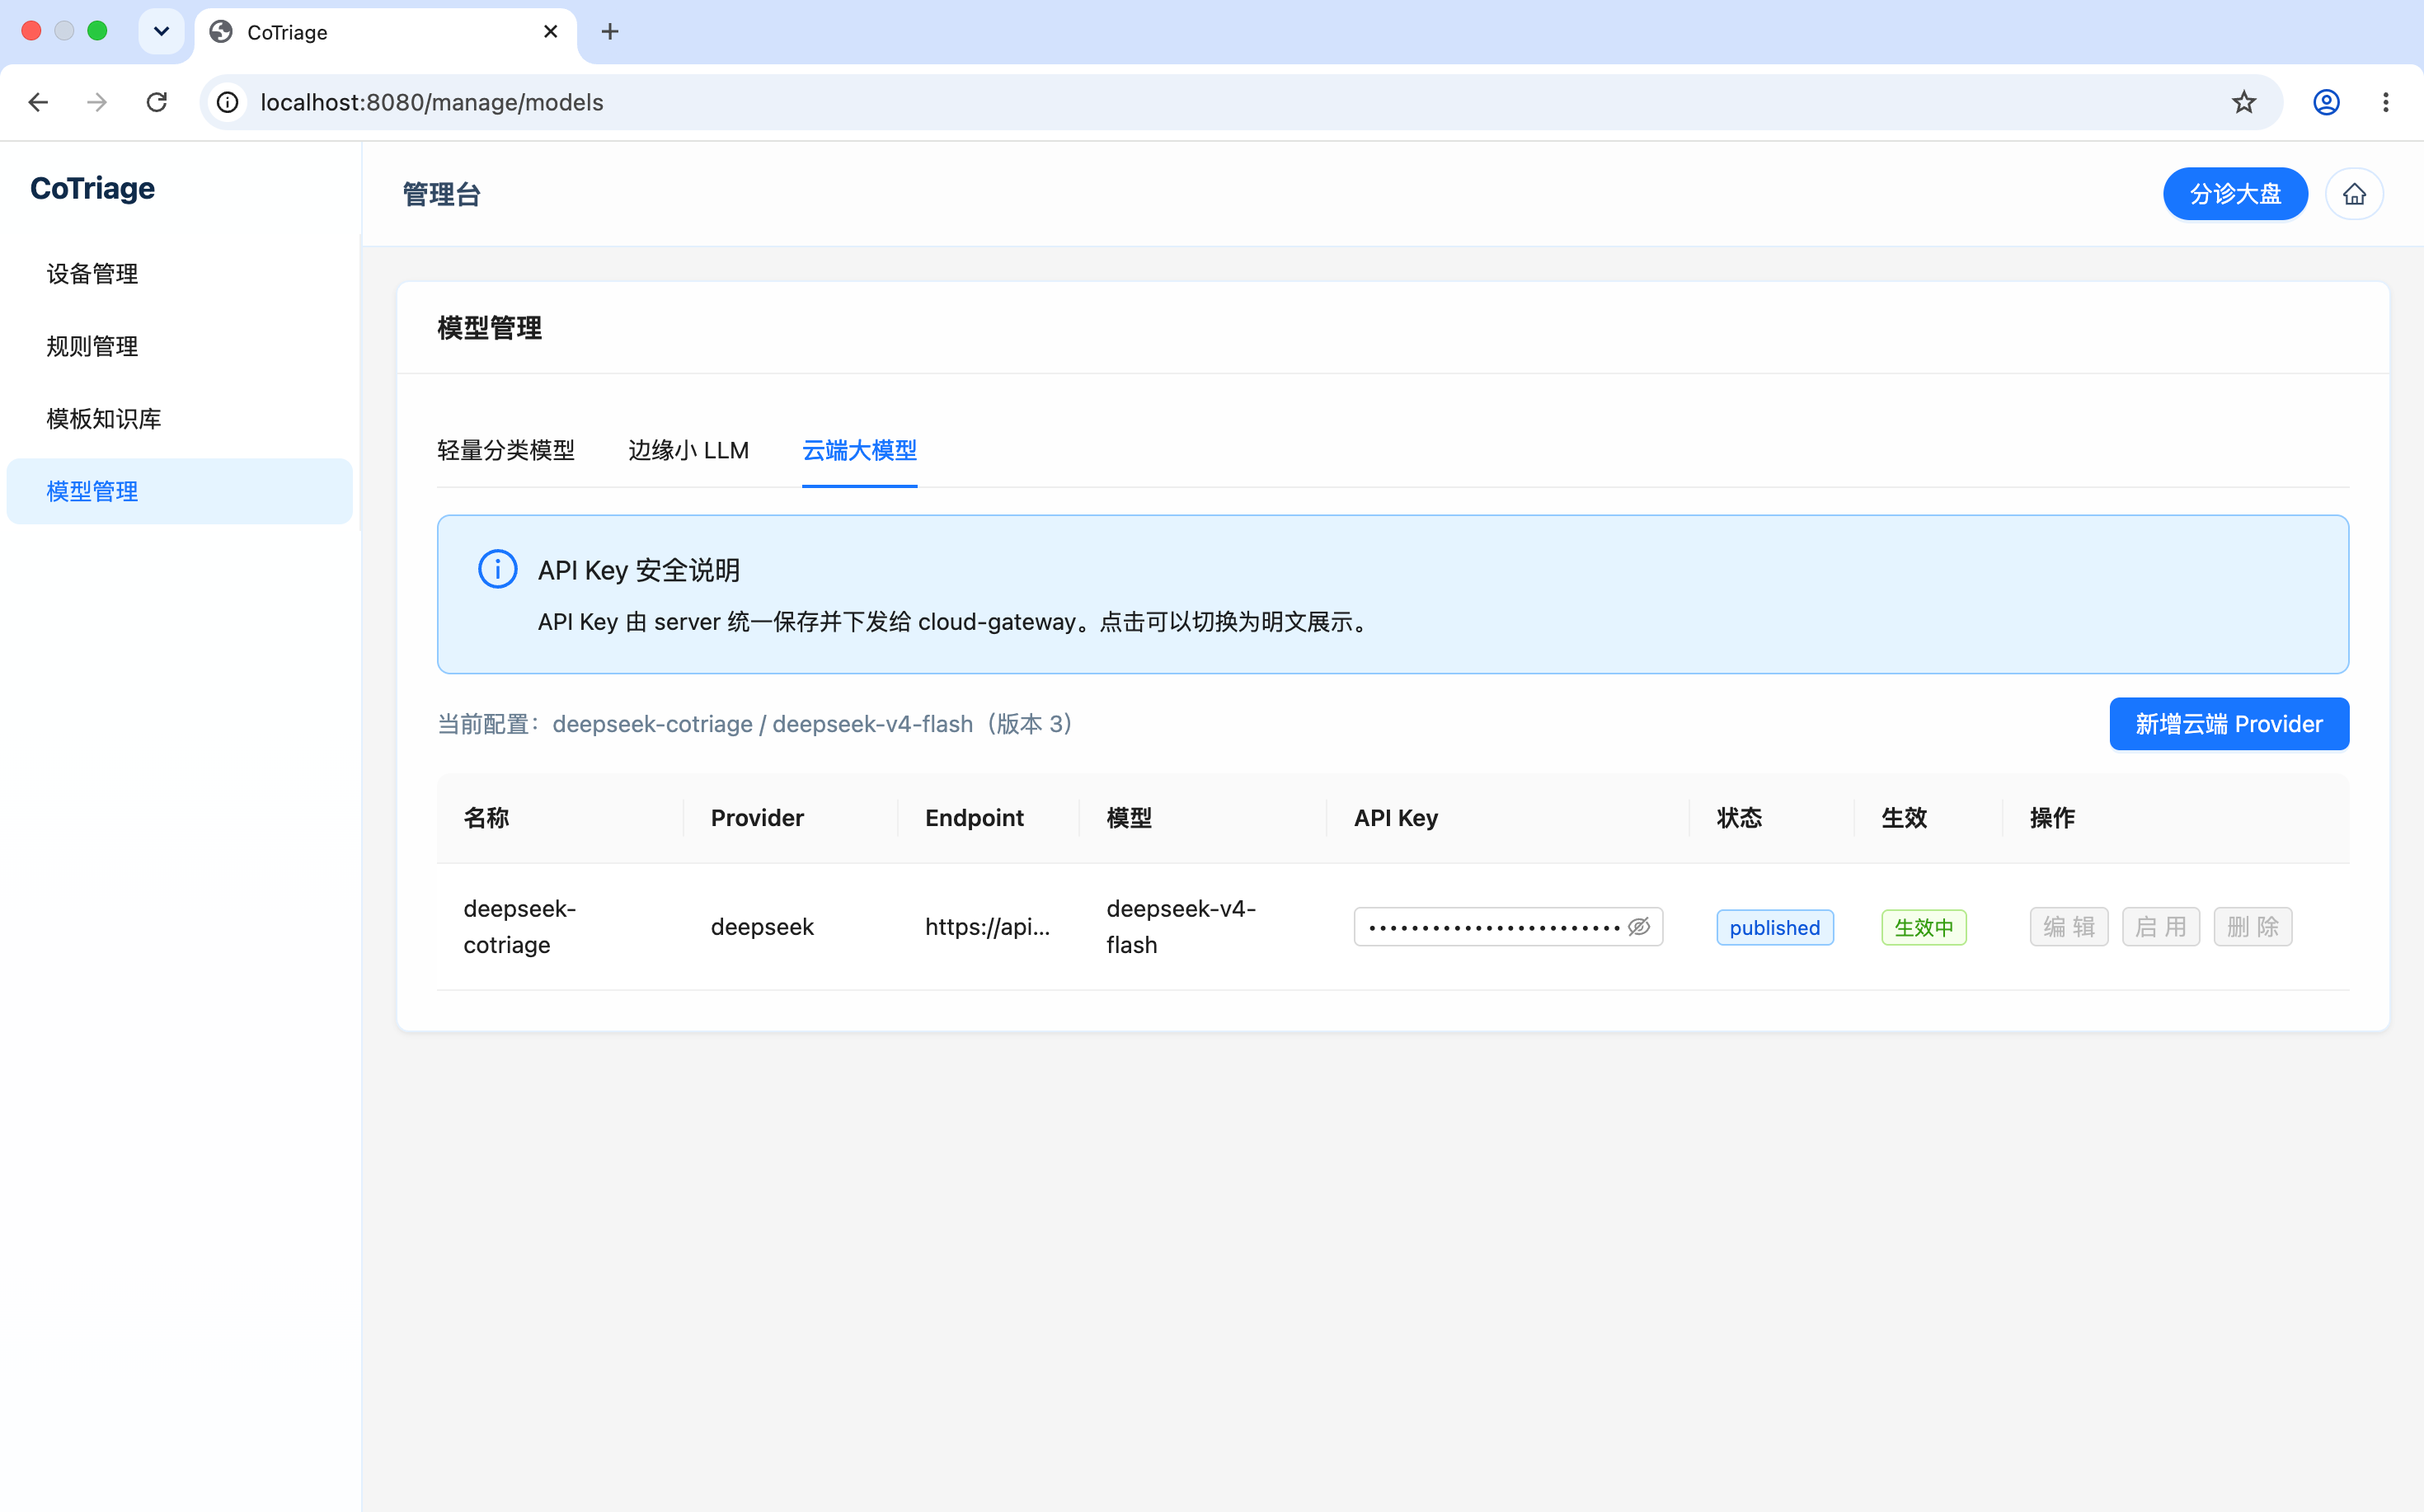
\includegraphics[width=0.96\textwidth]{figures/s-09c-cloud-provider-management.png}
  \caption{云端 Provider、模型参数、发布状态与密钥遮罩管理}
  \label{fig:cloud-provider-management}
\end{figure}

\cref{fig:cloud-provider-management}对应控制面的云模型配置实现。前端提交 Provider 名称、兼容接口地址、模型、超时、最大 Token 与密钥环境变量名；Server 校验后保存版本，Cloud Gateway 只读取当前活动且已发布的配置。

\section{Web 驾驶舱与实时交互实现}
\begin{figure}[htbp]
  \centering
  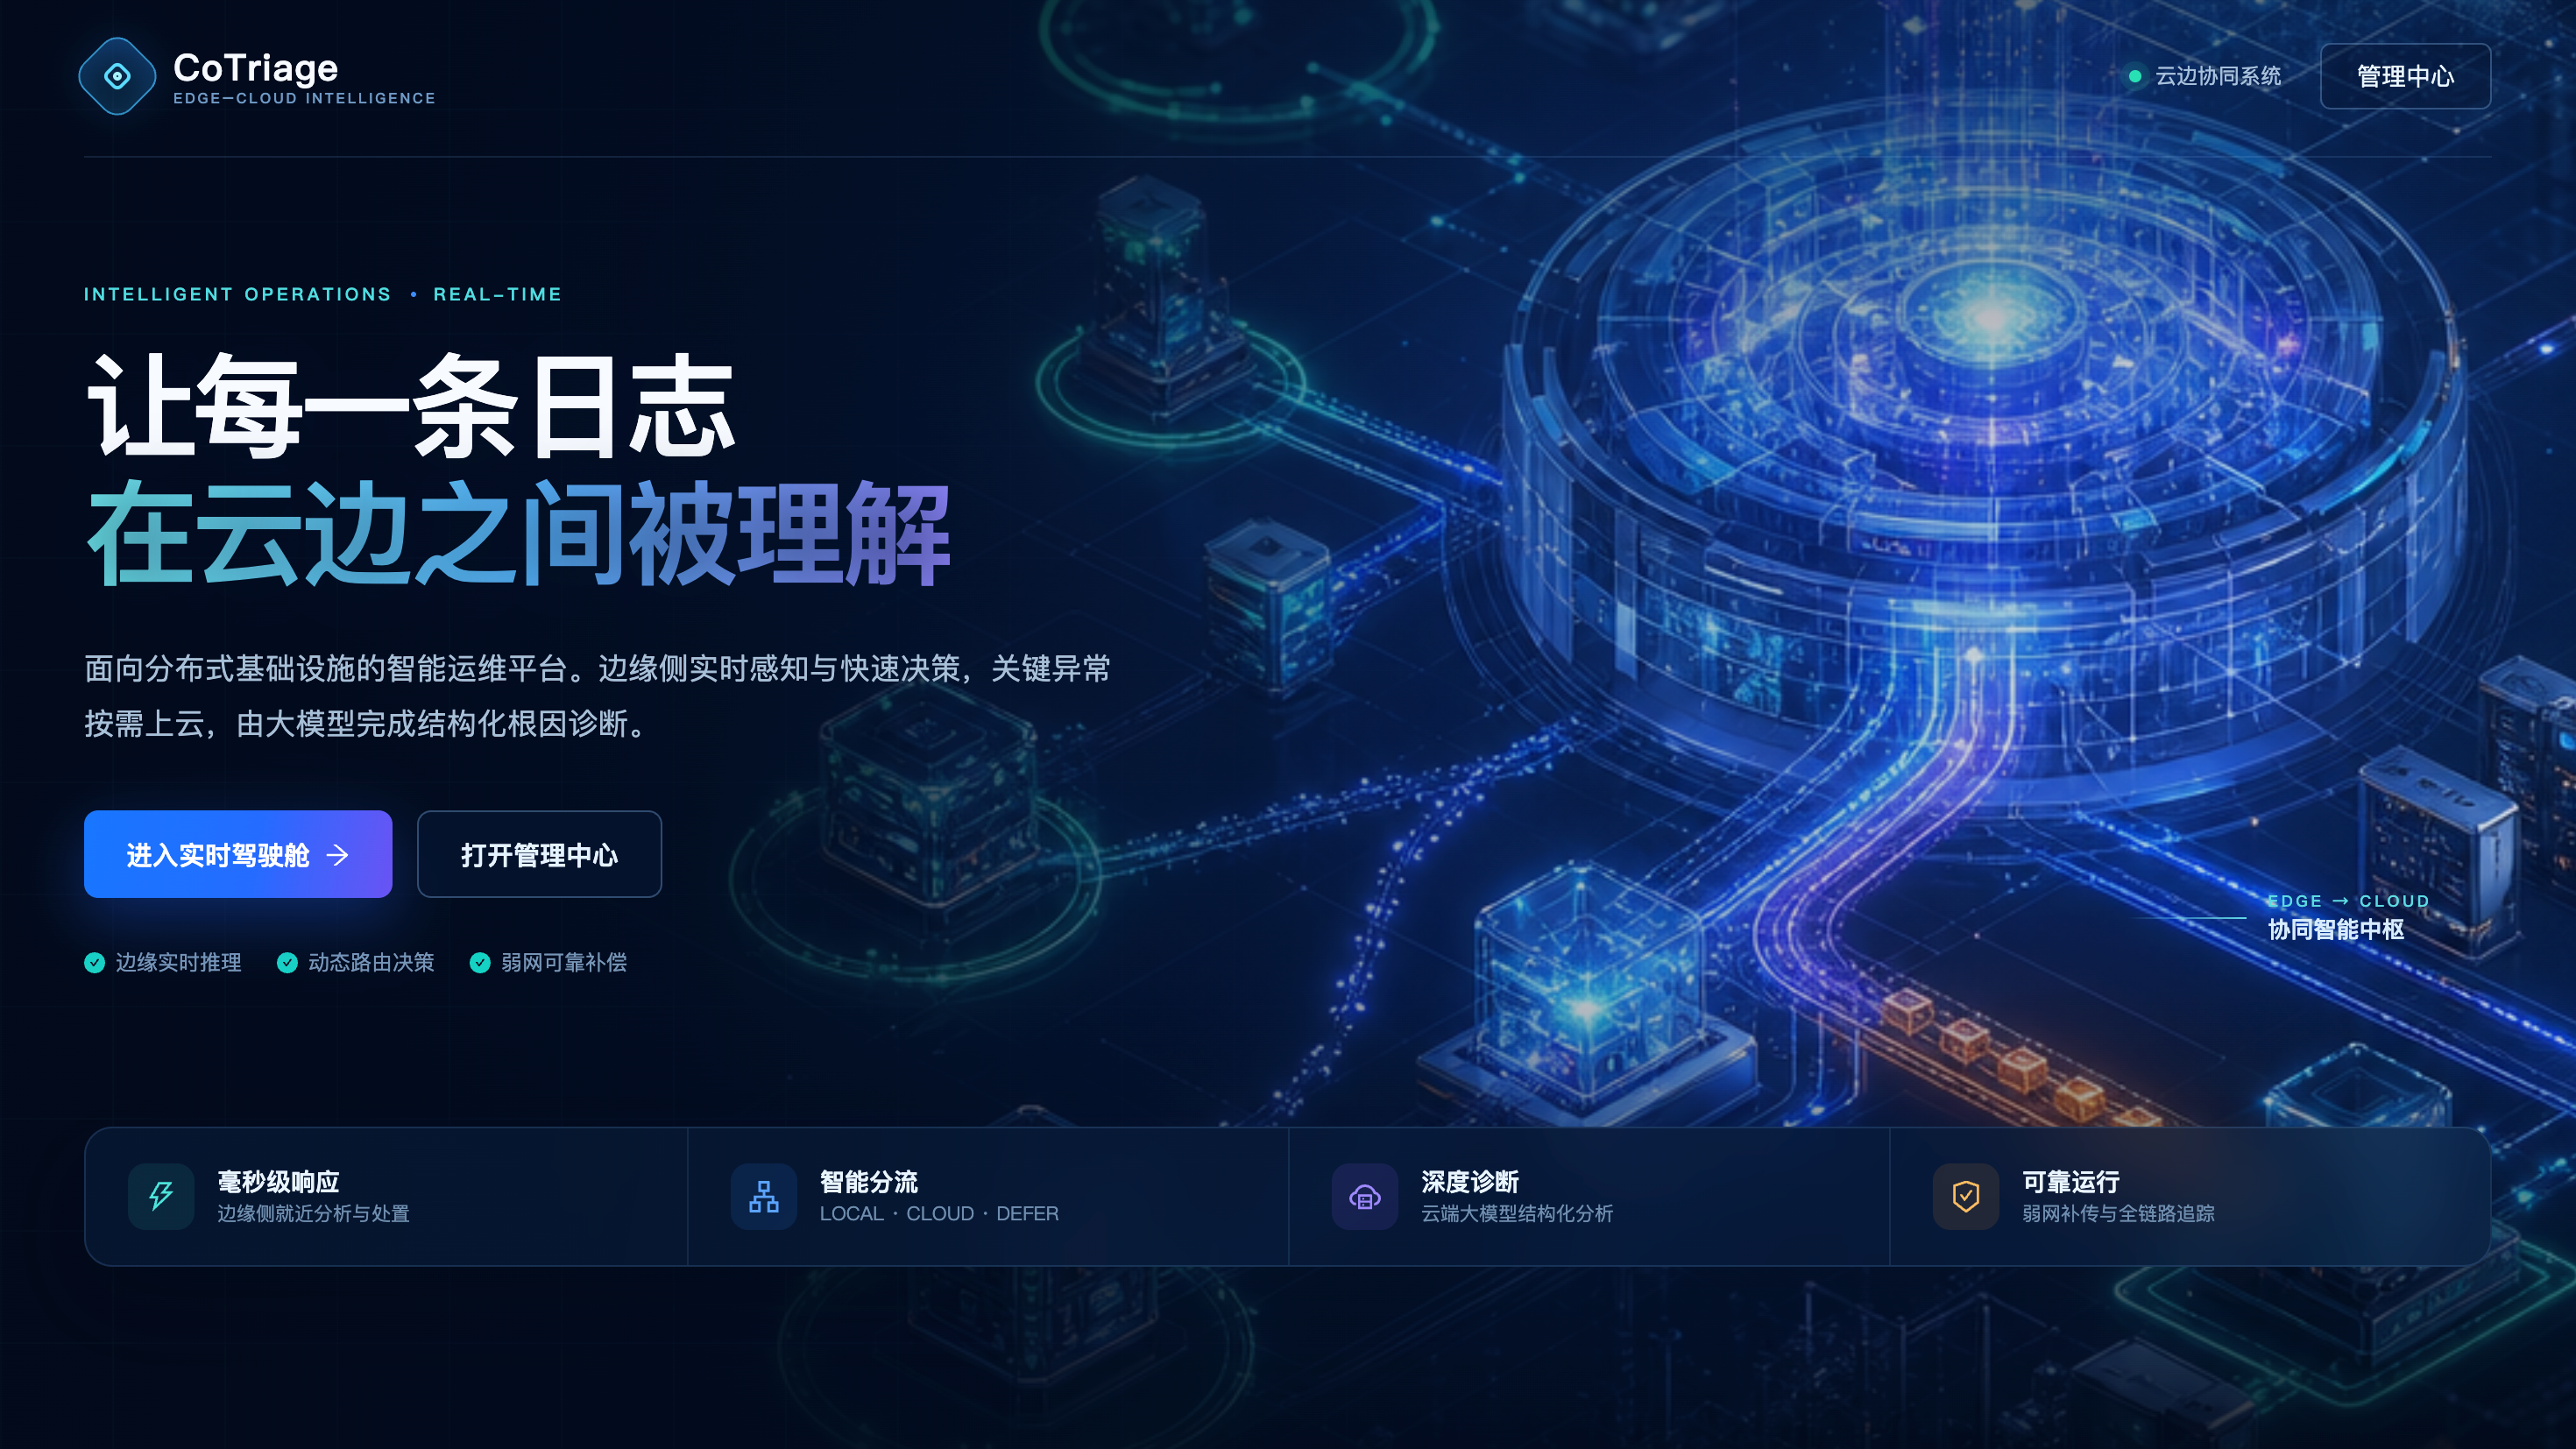
\includegraphics[width=0.98\textwidth]{figures/s-00-application-homepage.png}
  \caption{CoTriage 应用首页与核心能力入口}
  \label{fig:application-homepage}
\end{figure}

Web 使用 Vue 3、TypeScript、Vue Router、Ant Design Vue 和 ECharts 实现，由 Nginx 提供静态资源并将 \texttt{/api} 代理到 Server。\cref{fig:application-homepage}不是独立宣传页，而是产品导航入口：实时驾驶舱面向值守和演示，管理中心面向设备、知识和模型治理。

\begin{figure}[htbp]
  \centering
  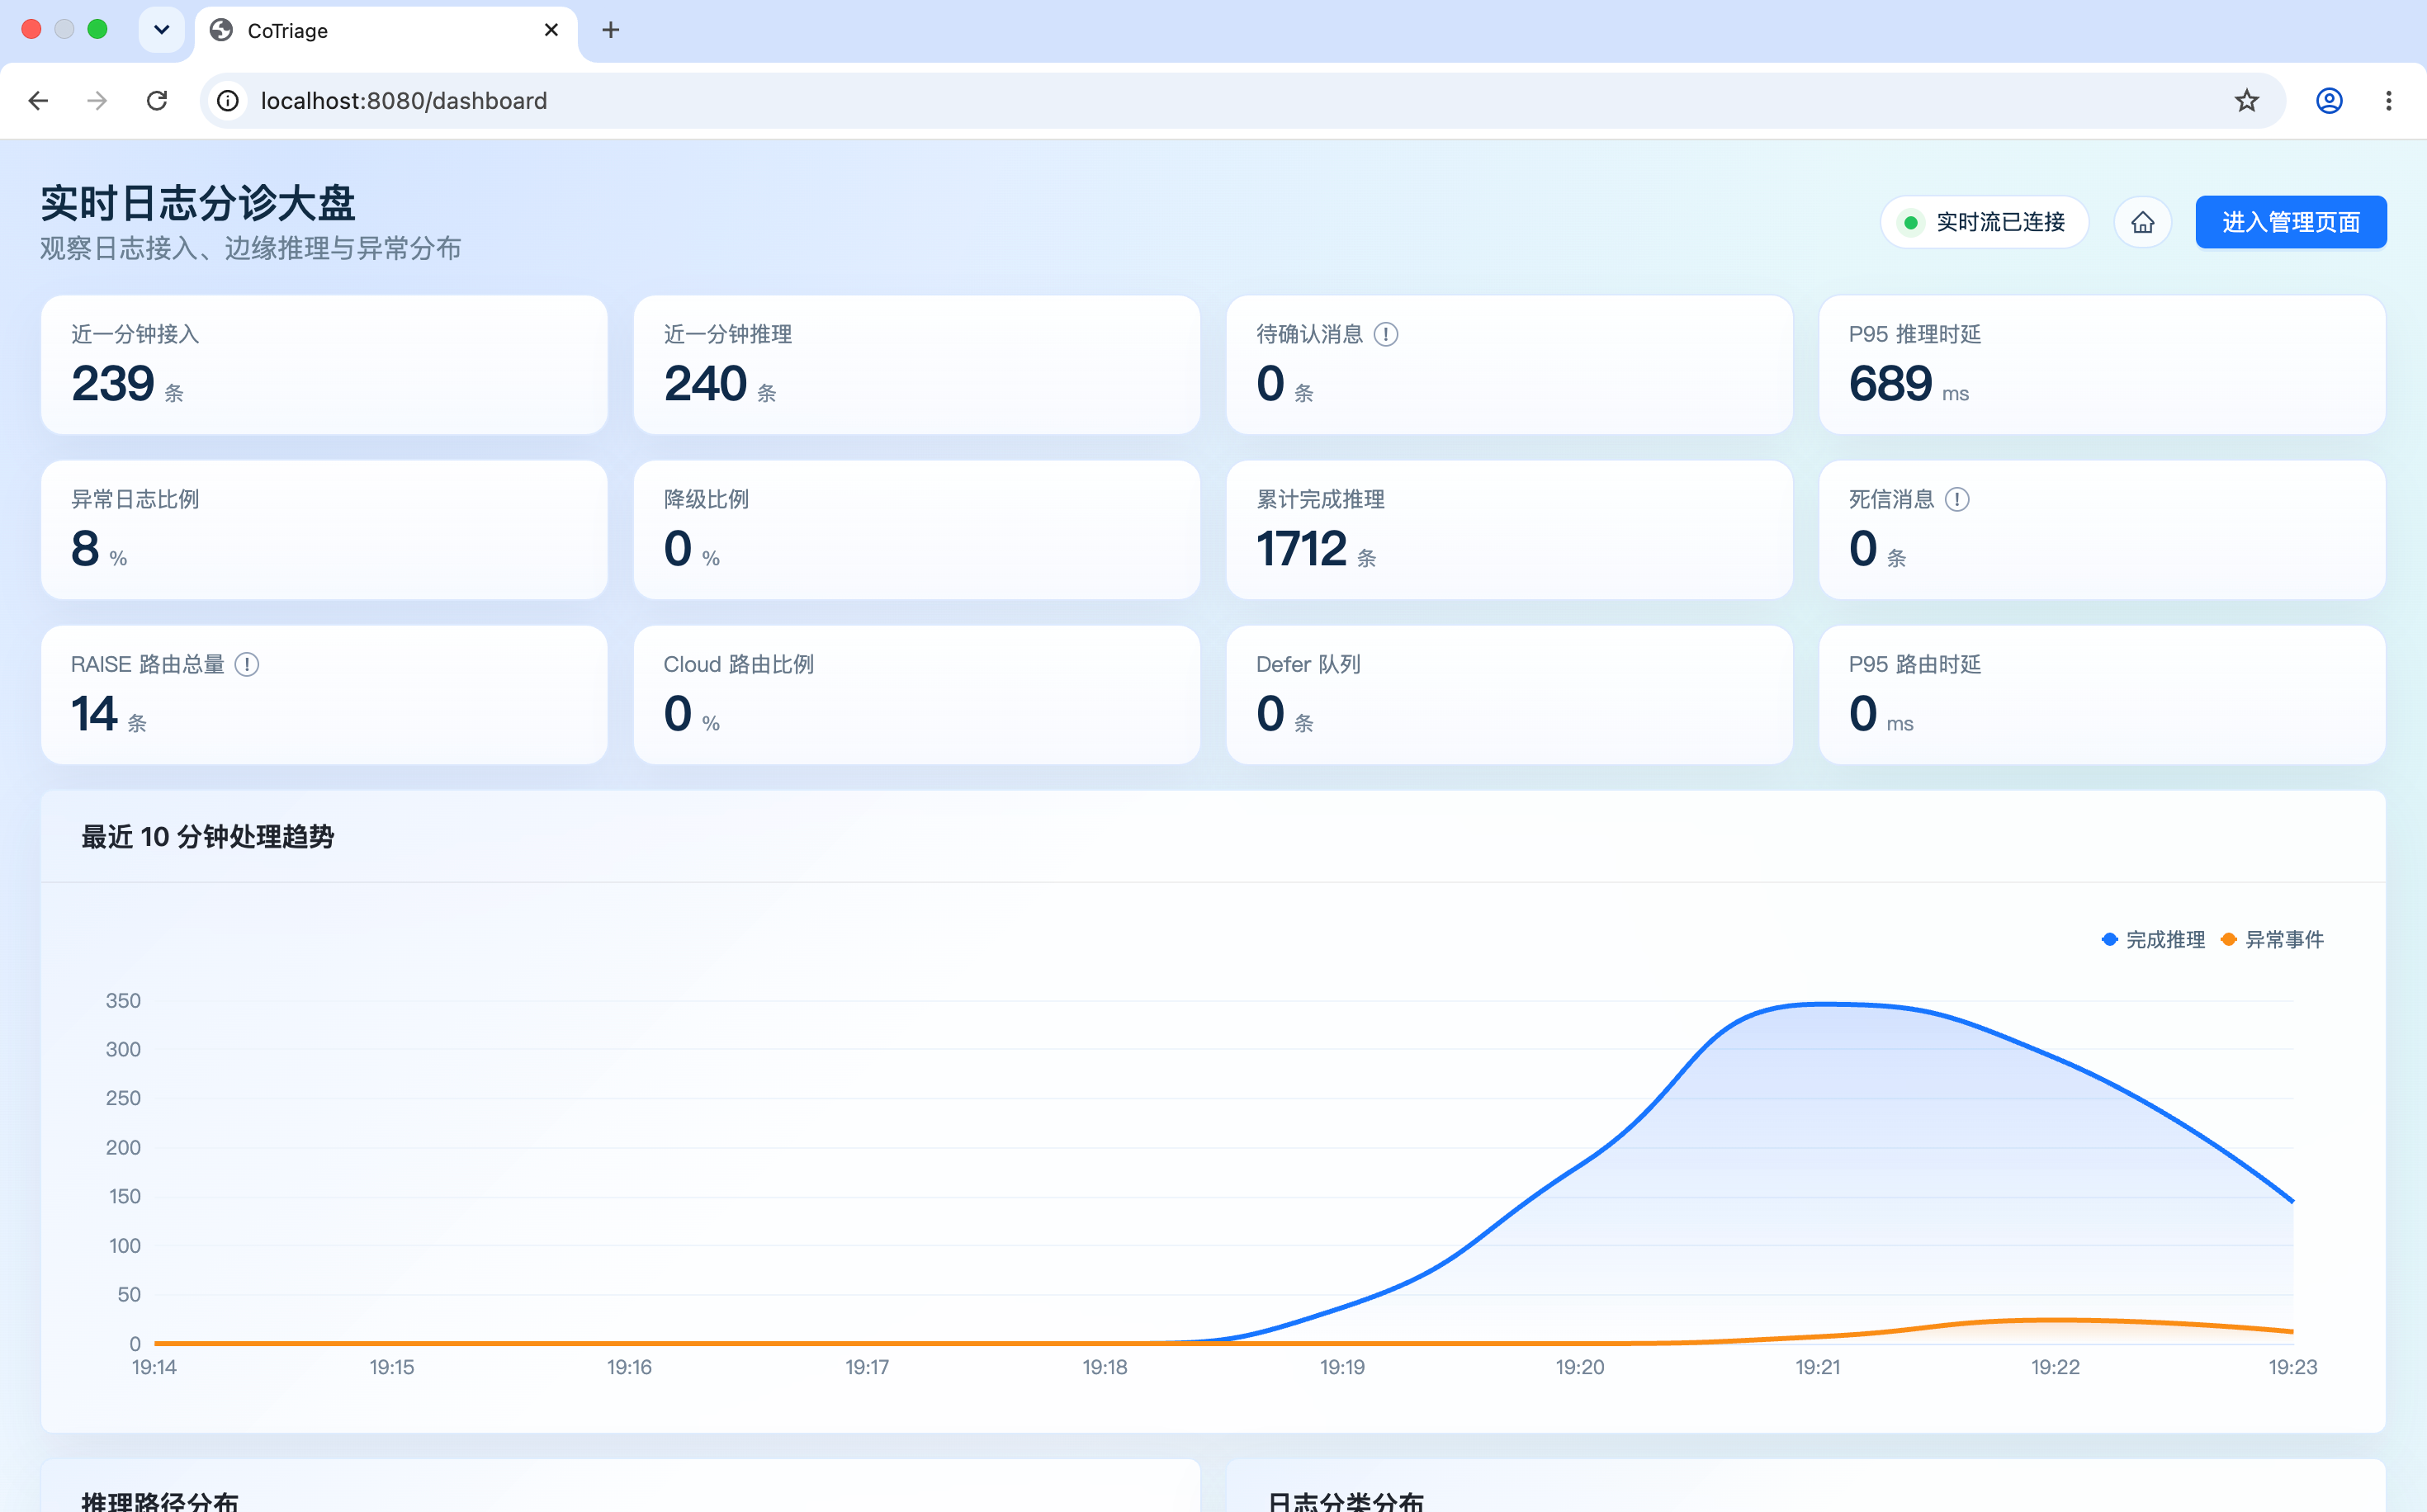
\includegraphics[width=0.98\textwidth]{figures/s-01-realtime-dashboard.png}
  \caption{REST 历史快照与 SSE 增量事件共同驱动的实时驾驶舱}
  \label{fig:realtime-dashboard}
\end{figure}

驾驶舱初始化时并行请求 summary、timeseries、abnormal-analysis、events、router summary、decisions、Outbox 和 cloud feedback，先形成一致的历史视图；随后建立 SSE 连接接收新事件，将增量数据合并到有限长度的本地数组中。连接断开时页面保留最后一次快照并进入重连状态，不会清空既有数据。用户可以暂停表格刷新，新事件暂存于缓冲区，恢复时批量合并，便于演示过程中展开某条事件而不被高频刷新打断。

页面围绕同一 \texttt{event\_id} 合并边缘事件、RAISE 决策和云端反馈。总览卡片显示接入、推理、异常、降级和路由状态；趋势图和分布图由 ECharts 响应式重绘；Outbox 区域展示状态、优先分数、尝试次数和错误；云端诊断只在根因、建议或解释字段存在时渲染相应内容，避免把不可解析占位信息展示给用户。事件表展开后显示原始日志、模板、推理证据、分阶段耗时、路由原因和云端诊断，从而把系统内部多阶段处理还原为一条可阅读的事件链。

\section{容器化部署、运维与安全实现}
\begin{figure}[htbp]
  \centering
  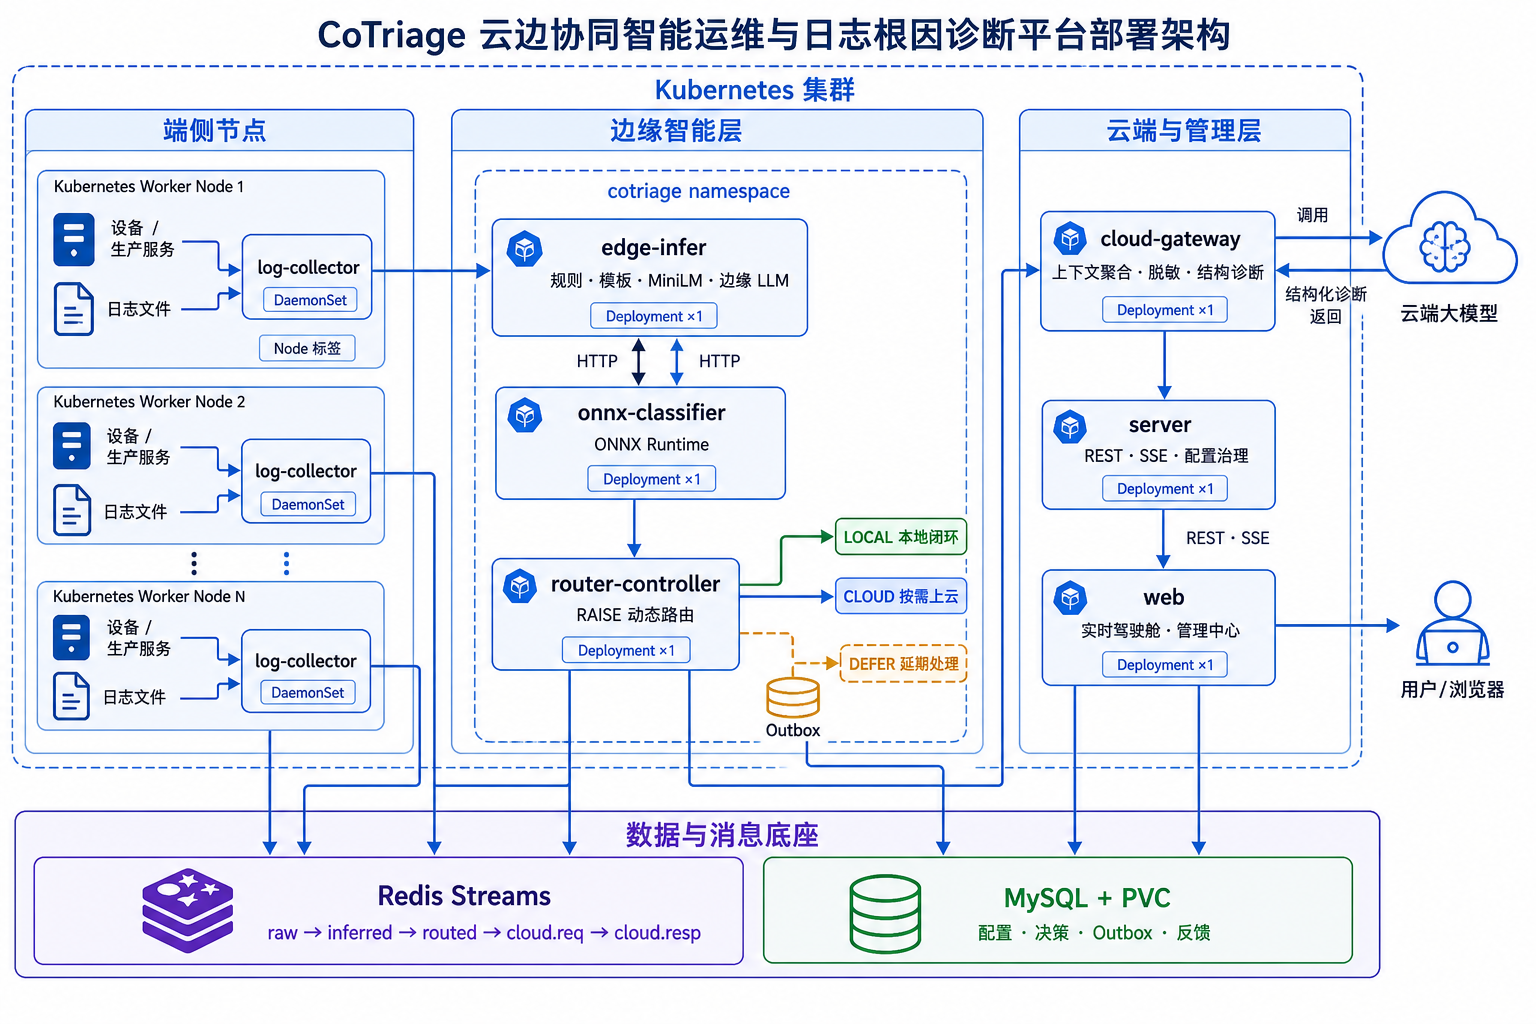
\includegraphics[width=0.98\textwidth]{figures/deployment-architecture.png}
  \caption{CoTriage 云边协同系统的 Kubernetes 部署架构}
  \label{fig:deployment-architecture}
\end{figure}

\cref{fig:deployment-architecture}给出了系统从端侧日志源、边缘智能处理到云端诊断与管理面的实际部署关系。端侧采集器以 DaemonSet 随节点部署，其余核心服务以单副本 Deployment 运行在 \texttt{cotriage} namespace；Redis Streams 承载阶段化事件流，MySQL 与 PVC 保存配置、决策、Outbox 和反馈等持久状态。云端大模型位于集群边界之外，仅由 Cloud Gateway 在路由动作选择 \texttt{CLOUD} 时按需调用。

仓库为主要服务提供独立 Dockerfile，并在 \texttt{charts/} 下维护 Kubernetes 资源。log-collector 采用 DaemonSet 贴近节点日志目录；edge-infer、onnx-classifier、router-controller、cloud-gateway、server 和 web 采用 Deployment；Redis 与 MySQL 通过 Service 暴露集群内地址并挂载 PVC。各业务组件通过 ConfigMap 或环境变量接收 Stream、超时、批次、并发和 RAISE 参数，敏感项由 Secret 或仅在进程环境中存在的变量提供。镜像可以独立构建并推送到阿里云镜像仓库，部署时限定在 \texttt{cotriage} namespace，服务间使用集群 DNS 而不是固定 Pod IP。

启动顺序首先确保 Redis、MySQL 和 ONNX 服务可用，再启动控制面、边缘推理、路由和云端网关，最后开放采集器与 Web。停止时先缩减采集入口，避免继续产生新事件，再等待或保留 Pending 与 Outbox。运行检查不仅关注 Pod 是否 Ready，还覆盖 Consumer Group Pending、Stream 长度、DLQ、MySQL 连接、Outbox 最老等待时间、云端 Provider 状态和 SSE 连接状态。组件使用 \texttt{SIGTERM} 派生的 context 结束读取循环，避免容器终止时继续接受新批次。

安全边界在实现中体现为三层：端侧通过节点标签和 ServiceAccount 最小权限识别来源；路由硬策略可禁止指定事件上云；Cloud Gateway 在构造提示词前执行脱敏和上下文裁剪。Provider 密钥不写入配置响应，管理页面只展示遮罩。对于生产环境，还需在现有基础上接入专用密钥托管、NetworkPolicy、字段级脱敏规则、访问审计和镜像签名，但这些扩展不会改变现有事件与组件接口。

综上，CoTriage 的工程实现不是若干模型接口的串联，而是一套围绕事件生命周期构建的分布式运行系统：实时路径以 Stream 和 Consumer Group 保证阶段解耦，知识与模型以版本配置实现在线治理，高价值任务以 Outbox 跨越弱网，云端结果以幂等反馈回写，控制面与驾驶舱则把内部状态转化为可操作、可解释的产品能力。
